
%%% Local Variables: 
%%% mode: latex
%%% TeX-master: t
%%% End: 

\chapter{研究背景}
\label{chap:background}

互联网应用如电子邮件、搜索、网络购物、社交网络、在线视频、网络地图等,已经成为人们生活的一部分。
这些应用往往要为上亿用户服务,意味着互联网应用已变成如电力一样的社会公共服务,
而支撑拥有海量用户互联网应用的数据中心也成为如同发电厂一样的社会核心基础设施。

长尾延迟(Tail Latency)问题在数据中心中受到越来越多的关注,
造成长尾延迟的原因有很多,其中最为重要的原因就是资源共享带来的干扰。
由于没有行之有效的方案对干扰进行控制,目前典型的数据中心都使用隔离的方式来减小干扰,
这一方案虽然有效缓解了长尾延迟,但它也带来了资源利用率过低的问题,
现有商用数据中心的资源利用率普遍只有10\%-30\%左右,造成极大的浪费。
如何解决服务质量与资源利用率的问题是当前业界面临的重大挑战。

本章内容安排如下:首先介绍新计算模式对数据中心的挑战,
然后讨论现有数据中心技术的局限性,即服务质量与资源利率冲突的原因,
之后介绍针对该问题的相关工作,主要是软件架构、资源调度和体系结构支持三个方面的工作。

%服务质量(QoS)与资源利用率是数据中心运营时需要考虑的两个重要指标,前者严重影响用户
%体验,而后者直接与数据中心的运营成本相关。然而现有的计算机体系结构并没有为服务质量
%保障提供足够的支持,造成这两个指标在现实状况下存在冲突。为了保障用户体验,在实际系
%统部署时,会更多的考虑服务质量这一指标,造成数据中心的资源利用率严重低下,普遍只有
%10\%-30\%左右。基于这一现状,本文主要讨论如何设计一种高效的数据中心体系结构,使得
%数据中心在保障应用服务质量基础上,达到较高的资源利用率。
%

\section{新计算模式对数据中心的挑战}

\subsection*{计算模式1:以云计算为基础的移动计算}

随着移动设备(平板电脑、智能手机)计算能力不断增强、成本不断降低以及无线通信技术的快速发展,
移动计算时代已经来临。
如表\ref{tab:ganter-sales}所示,Gartner调研数据显示平板电脑和手机(包含智能手机和普通手机)销量不断增加,
与此同时PC销量则不断下降。
而IDC预测到2015年智能手机销量将超过14亿部,占所有个人计算设备(包括PC、平板电脑和智能手机等)69\%的销量份额。

% Gartner关于电脑与移动设备销量的统计 
\begin{table}[htb]
  \centering
  \begin{minipage}[t]{0.9\linewidth}
  \caption[全球个人计算设备市场销量统计]{全球个人计算设备市场销量统计(单位:千部)}
  \label{tab:ganter-sales}
    \begin{tabular*}{\linewidth}{lrrrrr}
      \toprule[1.5pt]
      {\heiti 设备类型} & {\heiti 2012年} & {\heiti 2013年} & {\heiti 2014年} & {\heiti 2015年} & {\heiti 2016年} \\
      \midrule[1pt]
      PC(台式机、笔记本) &   341,273 &   296,131 &   279,000 &   259,000 &   248,000 \\ 
      超级本               &     9,787 &    21,517 &    39,000 &    62,000 &    85,000 \\ 
      平板电脑             &   120,203 &   206,807 &   216,000 &   233,000 &   259,000 \\ 
      手机                 & 1,746,177 & 1,806,964 & 1,838,000 & 1,906,000 & 1,969,000 \\ 
      其它移动设备         &       --- &     2,981 &     6,000 &     9,000 &    11,000 \\
      %总计                 & 2,217,440 & 2,334,400 & 2,378,000 & 2,470,000 & 2,572,000 \\
      \bottomrule[1.5pt]
    \end{tabular*}\\[2pt]
    \footnotesize
    数据来源:Gartner,2012年(http://www.gartner.com/newsroom/id/2610015),
    2013年(http://www.gartner.com-\\/newsroom/id/2791017),
    2014-2016年(http://www.gartner.com/newsroom/id/2954317)
  \end{minipage}
\end{table}

移动计算的快速发展带来新的计算模式:
移动设备通过无线通信与运行在云计算平台的各类应用服务进行交互。
据可靠消息,目前一些主要的互联网公司(如Facebook和Baidu等)均表示,
来自移动设备的请求已占到40\%以上,并且仍在快速增长,很快将超过PC。
随着4G时代的到来,这种移动计算模式将成为未来的主流。

快速增长的移动计算需求对云计算平台的核心——数据中心带来了严峻的挑战。这
种交互式计算模式,快速的服务响应时间是衡量服务质量(Quality-of-Service,QoS)的关键指标,
是让用户满意、留住用户的关键。有研究表明,如果服务响应时间增加,公司收入就会减少。
例如,2009年微软在Bing搜索引擎上也开展实验,发现当服务响应时间增加到2000ms时,
每个用户带给企业的收益更是下降了4.3\%。
由于该实验对公司产生了负面影响,最终不得不被终止\cite{bing:2009}。
Amazon也发现其主页加载时间每增加100ms就会导致销售额下降1\% 。
而Google更是发现当搜索结果返回时间从0.4s增加到0.9s时,广告收入下降了20\%。

\begin{figure}
\begin{minipage}{0.48\textwidth}
  \centering
  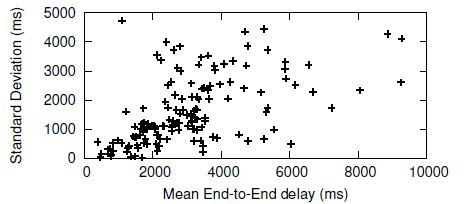
\includegraphics[height=5cm]{bg/end2end-delay}
  \caption[北美移动应用用户感知时延分布]{北美移动应用用户感知时延分布:平均延迟超过2秒且具有很大的波动性}
  \label{fig:end2end-delay}
\end{minipage}\hfill
\begin{minipage}{0.48\textwidth}
  \centering
  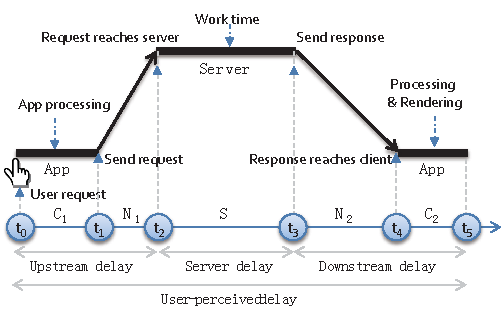
\includegraphics[height=5cm]{bg/interact-apps}
  \caption[一个典型的交互式请求的5个阶段]{一个典型的交互式请求的5个阶段:C1->N1->S->N2->C2 \cite{timecard:2013}}
  \label{fig:interact-apps}
\end{minipage}
\end{figure}

移动计算的响应时间仍然存在很大的提升空间。
如图\ref{fig:end2end-delay}所示,微软公司实验数据表明在北美网络环境下,
交互式移动设备的平均时延超过2秒,而且存在较大的波动性。
图\ref{fig:interact-apps}显示典型移动交互式应用的用户请求时延分为5个阶段,
最近研究\cite{timecard2013}表明其中数据中心服务器的处理时延S约为1.2秒,占60\%。
随着4G网络的来临,数据中心将面临更大规模用户数据的处理请求。
因此,如何快速处理和及时响应移动计算请求将成为数据中心设计的核心目标之一。


\subsection*{计算模式2:面向大数据处理的实时计算}

大数据时代的到来使大数据处理架构受到越来越多的关注。
2013年底中国计算机学会(CCF)大数据专家委员会发布的《2014年大数据发展趋势十大预测》 报告中,
来自学术界、产业界、海外、跨界特邀和政府的122位专家们普遍认为,
Hadoop/MapReduce框架一统天下的模式将被打破,而实时流计算、分布式内存计算、图计算框架等将并存。

\begin{figure}[H]
  \centering
  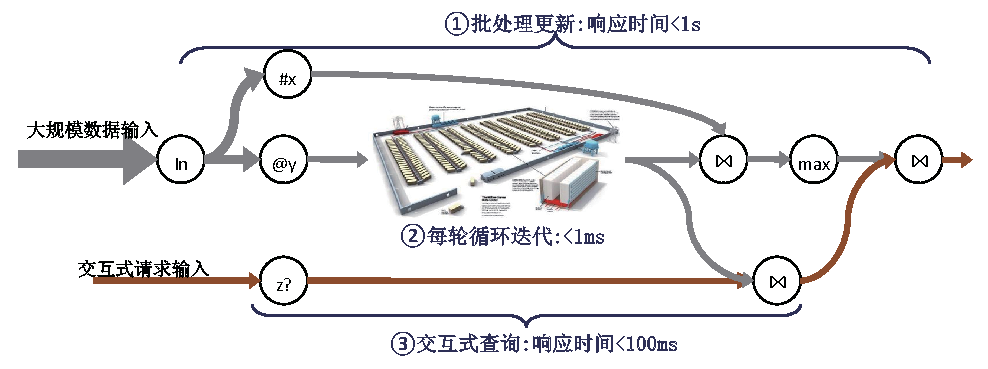
\includegraphics[height=6cm]{bg/batch-apps}
  \caption{典型的3类大数据处理需求以及相应的响应时间要求}
  \label{fig:batch-apps}
\end{figure}


大数据处理对数据中心和处理架构提出新的挑战,
图\ref{fig:batch-apps}显示了典型的大数据处理需求:
首先需要支持数据的批处理更新模式(<1s);
其次数据处理会分解为多次迭代计算(<1ms);
再次还要支持实时计算模式,处理多用户的交互式查询请求(<100ms);
而这些处理所需要的数据存放在同一个数据中心。
搜索引擎是一个典型的例子,既需要对大规模网页进行内容处理,迭代计算页面的pagerank,
还需要处理大量用户的关键字查询请求。

尽管大数据处理希望能将各种处理集成在一个处理架构上,然后部署在一个数据中心。
但如果实时计算与企业营收相关,比如搜索引擎、在线购物等在线服务应用,
那么正如微软Bing实验所示,这些面向在线服务应用的实时计算的服务质量就非常关键(以下用“在线应用” 代表“实时计算”)。为了
保障在线应用的服务质量,主流互联网企业一般将在线应用与大规模批处理作业分别部署到不同的数据中心,
以减少批处理作业对在线应用的干扰。
但由于用户查询请求数量具有显著的随时间变化的波动性,
这种分离作业、单独部署的模式会导致在线应用数据中心的资源平均利用率很低。
如图\ref{fig:google-util-2013}所示,Google的两类数据中心CPU利用率相差达2.5倍,在线应用数据中心资源利用率仍有很大提升空间。


%% 典型的数据中心一般有5~10万台服务器组成,建设与运行维护成本往往高达几十亿人民
%% 币。然而出于保障应用服务质量的原因,现有数据中心只能维持较低的资源利用率,导致大量
%% 资源浪费。因此,本项目总体研究目标为如何设计高效通用数据中心体系结构:“通用”表
%% 示数据中心可同时运行各种不同类型应用;“高效”表示数据中心能在保障延迟敏感应用的服
%% 务质量基础上,达到较高的资源利用率(CPU利用率>60\%)。
%% 
%% 典型的数据中心一般有5~10万台中低端服务器组成,这些服务器通过内部网络互连,一起协同
%% 运行互联网应用为海量用户服务。因为这类数据中心规模很大,往往部署在大型仓库级别的机
%% 房,从应用角度来看就如同一台计算机,因此也被称为
%% “仓库级计算机(Warehouse-Scale Computer)“ \cite{WSC}。
%% 国内外著名的互联网公司往往拥有多个数据中心,服务器数量达到数十万甚
%% 至上百万台。例如,谷歌(Google)的数据中心服务器数量已经超过百万台为全球用户提供
%% 搜索、邮件、地图等服务[2];亚马逊(Amazon)仅EC2就部署了约50万台服务器提供云计算服
%% 务[3];据可靠消息,国内腾讯公司也拥有约30万服务器为用户提供各种互联网服务。
%% 
%% 尽管目前互联网企业的数据中心已经颇具规模,但一个趋势是未来数据中心还将持续发展。一
%% 方面互联网用户数量仍在不断增长,目前全球已有24亿网络用户,但很多机构预测未来全球还
%% 将新增30亿网民融入到互联网[4],这会对数据中心的数量和规模都提出更多需求。另一方面快
%% 速发展的移动终端已超越个人计算机(PC),成为终端计算设备的主流。由于移动设备性能相对
%% 较低、存储容量较小,将计算与存储转移到数据中心的需求也变得越来越强烈。因此数据中心作
%% 为基础设施也会日益重要。


\section{现有数据中心技术的局限性}

通过上述分析可知,移动计算与实时计算均对快速响应用户请求提出了强烈的需求。
而当前数据中心为了保障用户请求的服务质量,不得不通过采用牺牲资源利用率、保留过量资源的方式。
Google的数据中心技术一直处于领先地位,我们以Google为例分析数据中心资源利用率现状。
图\ref{fig:google-util-2006}显示了2006年Google数据中心平均CPU利用率为30\%左右。
但到2013年,虽然Google将数据中心分为了两类,并且批处理数据中心已经能达到75\%的CPU利用率,
但在线应用数据中心仍停留在30\%。
我们对国内企业调研发现,几大主流互联网企业在线应用数据中心CPU利用率一般都低于20\%,
有的甚至低于10\%,仍然存在很大的提升空间。

% Google数据中心利用率 
\begin{figure}
\begin{minipage}{0.57\textwidth}
  \centering
  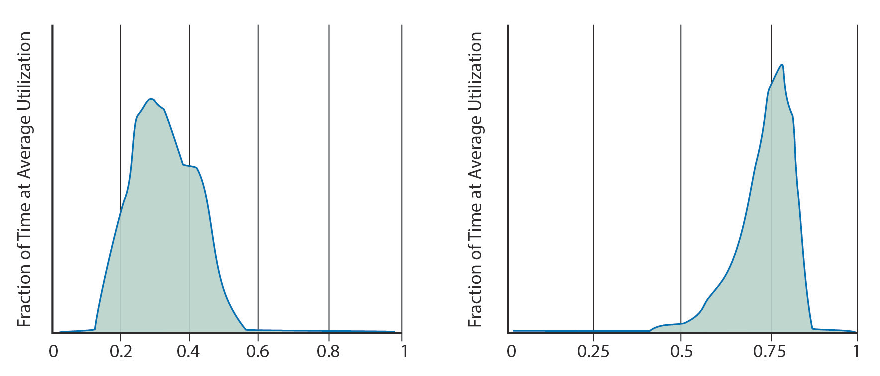
\includegraphics[height=4cm]{bg/google-util-2013}
  \caption[Google数据中心CPU利用率分布(2013年)]
    {Google数据显示2013年1至3月在线应用数据中心CPU利用率平均只有30\%(左图),
     而批处理作业数据中心则能达到75\%的利用率(两个数据中心均为2万台服务器)}
  \label{fig:google-util-2013}
\end{minipage}\hfill
\begin{minipage}{0.39\textwidth}
  \centering
  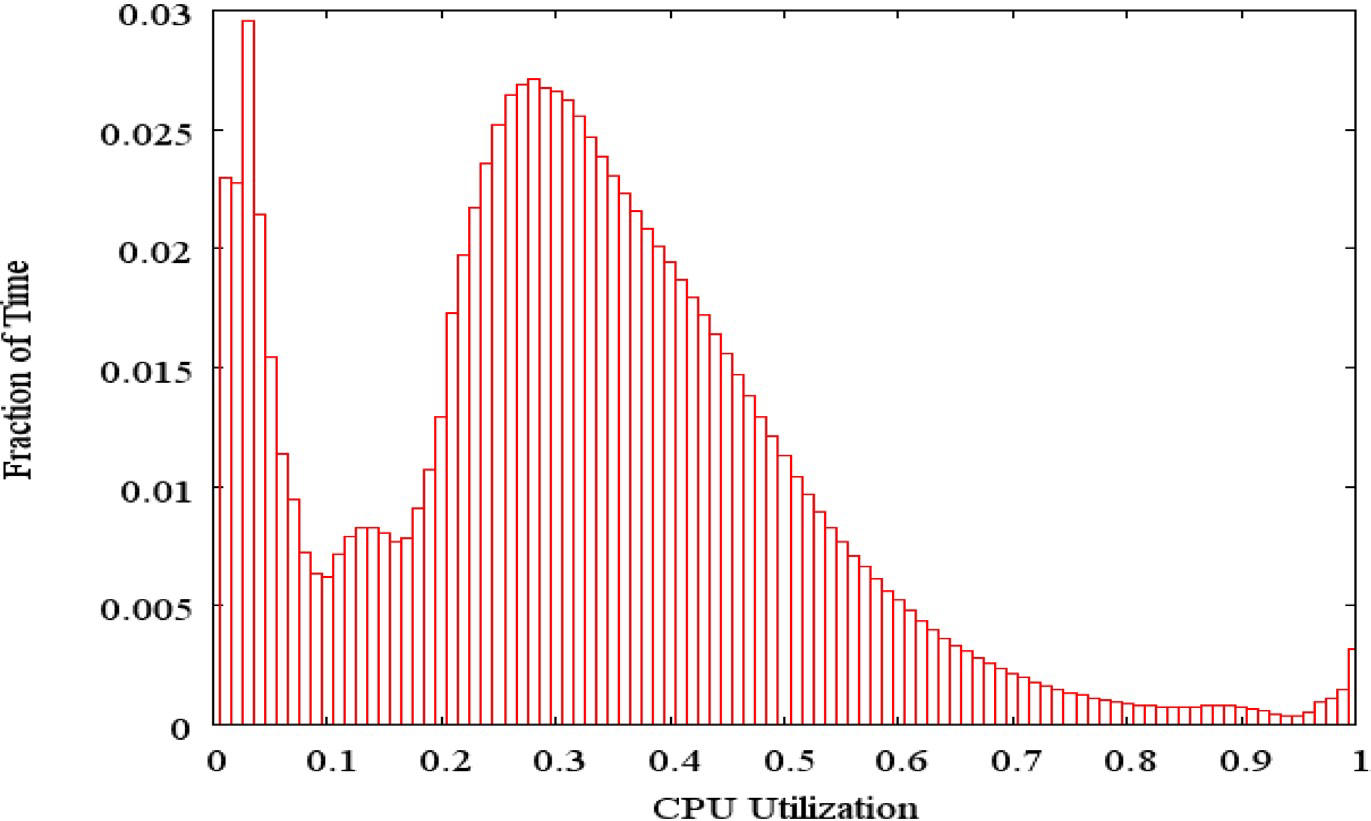
\includegraphics[height=3.5cm]{bg/google-util-2006}
  \caption[Google数据中心CPU利用率分布(2006年)]
    {Google在2006年数据中心(5000台服务器)6个月的CPU利用率分布}
  \label{fig:google-util-2006}
\end{minipage}
\end{figure}

尽管在线数据中心资源利用率只有30\%,但Google已经观察到严峻的长尾延迟现象:
最慢的1\%~10\%请求处理时间远大于所有请求的平均响应时间。
如图\ref{fig:google-resptime-dist}所示,Google某后台服务延迟响应时间平均仅为5~6ms,
但是却有相当一部分请求响应时间超过了100ms\cite{Krushevskaja:2013}。
而长尾延迟现象在数据中心环境下会被更进一步放大,
因为一个用户请求需要几百上千台服务器共同完成,只要有一台服务器的处理速度受到干扰,
就会导致整个请求的处理时间增加。
Google的Jeff Dean在2012年Berkeley的报告\cite{dean_achieving_2012}中就指出了长尾现象的严重性,
假设一台机器处理请求的平均响应时间为1ms,
有1\%的请求为长尾处理时间会大于1s(99th-Percentile)。
如果一个请求需要由100个这样的节点一起处理,
那么就会出现63\%的请求响应时间大于1s
(如图\ref{fig:long-tail-amplify}所示)。

造成在线应用数据中心资源利用率低和长尾延迟现象的核心原因是,
现有数据中心技术无法在多应用混合运行时消除应用间干扰,以实现不同应用之间的性能隔离。
Google的Jeff Dean与Luiz Barroso在2013年2月的《Communication of the ACM》上撰文
“The Tail at Scale”\cite{dean_tail_2013}分析确认导致长尾延迟的首要原因就是资源共享,
包括体系结构层次的CPU核、Cache、访存带宽、网络带宽等,而干扰不仅来自应用,
还会来自系统软件层次的后台守护作业、监控作业、共享文件系统等。
Google在分布式架构和软件层次采用了多种缓解长尾延迟的技术,
包括操作系统容器隔离技术\cite{cgroup}、应用优先级管理\cite{google_trace}、
备份请求\cite{dean_achieving_2012}、同步后台管理进程\cite{dean_achieving_2012}等,
取得了一定的效果,但却无法消除硬件体系结构层次上的应用之间的干扰,
导致仍然会出现图\ref{fig:google-resptime-dist}这样的长尾延迟。

\begin{figure}
\begin{minipage}{0.44\textwidth}
  \centering
  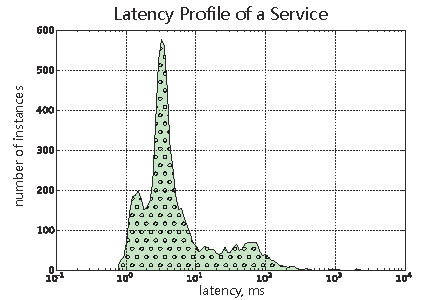
\includegraphics[width=\textwidth]{bg/google-resptime-dist}
  \caption[Google某后台服务的响应时间分布]{Google某后台服务的响应时间分布\cite{Krushevskaja:2013}}
  \label{fig:google-resptime-dist}
\end{minipage}\hfill
\begin{minipage}{0.52\textwidth}
  \centering
  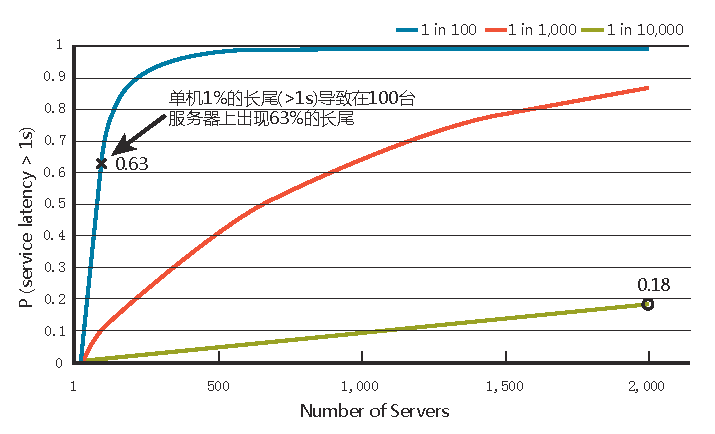
\includegraphics[width=\textwidth]{bg/long-tail-amplify}
  \caption[长尾延迟放大效应]{长尾延迟放大效应\cite{dean_tail_2013}}
  \label{fig:long-tail-amplify}
\end{minipage}
\end{figure}

因此,现有数据中心处于“无管理的资源共享”状态,这
导致出现资源利用率与应用服务质量之间的矛盾:
一方面通过多个应用同时在数据中心部署实现资源共享能有效提高资源利用率,
但另一方面多个应用共享资源又会出现相互干扰严重影响应用的服务质量。
因此,目前企业不得不采用预留额外资源以保障延迟敏感的在线应用服务质量,
这导致很低的数据中心利用率。
而且随着多核技术的发展,单个服务器内的资源越来越多,
其上混合部署的应用数目也在不断增加,更会加剧这种矛盾。

\section{相关工作}

随着应用数量与规模的不断增加,数据中心所需要的服务器数量也在飞速增长中。
而受到电力供应、冷却系统以及占地面积等客观因素的影响,
服务器规模并不能够无限制的扩大,
服务器融合(Server Consolidation)成为当前应用部署的主流技术。
本节首先介绍当前常见的服务器融合技术,并对比其在资源、性能等方面的隔离性;
然后介绍在这种服务器融合的共享环境下,已有的服务质量与资源管理的相关工作;
最后对比网络领域中解决服务器质量与资源管理的方案,
讨论将其应用于计算机体系结构中的可行性。

\subsection{服务器融合技术}

通过考查现代数据中心的应用架构,可以发现其中大部分架构都符合“数据复用模型”,
即多个应用程序协同工作,每个应用只对数据进行部分处理,然后交给下级应用程序,
这些应用程序最终组合完成一个服务功能,提供给最终用户。
通过这种方式形成的复杂应用架构,由于在兼容性、性能或安全等多方面的原因,
各个模块通常不能很好的在一台服务器内工作,而是需要多台服务器进行部署,
大量这样的多服务器应用给数据中心的维护工作带来了很大的挑战。
从另一方面,应用与服务器规模的不断增长,
数据中心在占地、电力消耗、冷却系统等方面也产生了极大的压力,
但服务器资源利用率过低的问题,造成数据中心整体的效率十分低下。
为解决这一问题,许多软硬件厂商都提出了自己的方法与技术,
将应用部署到更少的物理服务器中,实现高效可管理的服务器融合,
其中虚拟化、硬件分区与基于容器的轻量级虚拟化是三种目前应用最为广泛的服务器融合技术。

%软件虚拟化
虚拟化技术最初由IBM在20世纪60年代提出,当时提出虚拟化的目的是为了提供系统的向后兼容性,
以简化用户编程。而后,虚拟化一直是大型机使用的基本方式。
VMware首先将虚拟化技术引入到基于x86的PC服务器领域,
由于当时x86架构并没有提供任何虚拟化的支持,
VMware使用二进制翻译\cite{}的方式实现操作系统内核中不支持虚拟化的指令执行,
如图\ref{fig:compare-of-virt}(a)所示,实现对用户操作系统透明的虚拟化方案。
这种基于二进制翻译的全虚拟化方案性能存在问题,
因此Xen提出了半虚拟化(para-virtualization)\cite{barham_xen_2003}的概念,
通过修改客户机操作系统,直接使用Hypercall的方式调用hypervisor
(如图\ref{fig:compare-of-virt}(b)所示),实现部分功能,提高系统性能。
在虚拟化产业发展起来后,各个硬件厂商分别推出新的硬件功能以更好的支持虚拟化,
如Intel的VT-x技术和AMD的AMD-V技术,都在现有的体系结构下增加了根特权级,
也支持虚拟化操作,如图\ref{fig:compare-of-virt}(c)所示。
同时,其它一些用于提高虚拟化性能的硬件技术,如EPT、VPID、虚拟化I/O-APIC等,
也逐渐被开发出来,随着虚拟化技术性能的不断提高,当前在PC服务器领域,
虚拟化技术已经成为数据中心内被普遍使用的技术。

\begin{figure}[t]
  \centering
  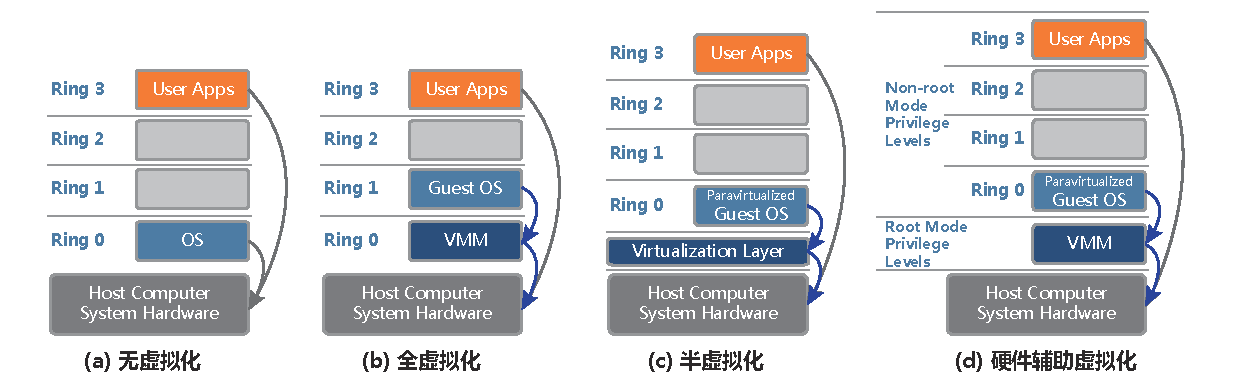
\includegraphics[width=\textwidth]{bg/compare-of-virtualization}
  \caption[三种不同类型虚拟化技术的对比]{三种不同类型虚拟化技术的对比:
    (a)无虚拟化,直接执行用户与OS请求;
    (b)全虚拟化,直接执行用户请求,二进制翻译执行OS请求;
    (c)半虚拟化,直接执行用户请求,修改GuestOS通过Hypercall实现特权指令;
    (d)硬件辅助虚拟化,直接执行用户请求,硬件支持OS特权指令直接陷入到VMM。}
  \label{fig:compare-of-virt}
\end{figure}

%硬件虚拟化
软件虚拟化技术其主要问题是开销,因于需要Hypervisor的干预。
早期大型机所使用的分区技术是另一种硬件方案,在硬件上支持分区,如IBM的LPAR\cite{},
SPARC系统的Logical Domain\cite{},

%轻量级虚拟化
为了降低虚拟化开销,出现容器技术,如Docker\cite{}和Rocket\cite{}都是基于容器技术的实现。
图\ref{fig:docker-overview}给出了Docker的架构,可以

\begin{figure}[H]
  \centering
  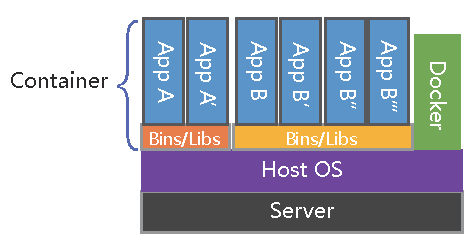
\includegraphics[width=0.5\textwidth]{bg/docker-overview}
  \caption[容器虚拟化结构示意(Docker)]{容器虚拟化结构示意(Docker):
    容器之间共享操作系统内核,但应用、运行时环境是隔离的}
  \label{fig:docker-overview}
\end{figure}

%各种服务器融合技术对比


\subsection{资源管理与服务质量保障}

Table \ref{tab:contention} illustrates prior work on eliminating contention at various layers.
Companies like Google and Twitter now adopt advanced data center management frameworks
(e.g., Borg\cite{borg:2015}, Omega \cite{Schwarzkopf_omega_2013}
and Mesos \cite{Hindman:2011:Mesos}) to balance the trade-offs between
resource utilization and applications' QoS.
There are also a number of distributed techniques and OS kernel
optimizations, such as multi-level priorities \cite{google_trace},
scheduling \cite{delimitrou_paragon:_2013, delimitrou_quasar:_2014,  mars_heterogeneity_2011,
kozyrakis_reconciling_2014, Novakovi:ATC2013}, backup-request \cite{dean_tail_2013},cgroup \cite{cgroup},
and resource containers \cite{lxc}.

Instead of presenting related work of all layers, in this section we focus on related work within a server.

\textbf{软件划分技术} 页着色技术(page coloring)是一种以软件方式控制内存物理页映射的方法,
通常被用作共享末级缓存与DRAM的划分,其核心思路是通过控制地址映射信息实现硬件资源的管理。
Lin和Tam等人提出基于页着色技术的缓存容量划分,以及解决缓存竞争问题
基于该技术可以实现对共享末级缓存和DRAM的划分,

Researchers propose to leverage
page-coloring technique to partition cache and DRAM.
The key idea of page coloring is leveraging address mapping information to manage hardware
resources.
Lin \emph{et al.} \cite{lin_gaining_2008}
and Tam \emph{et al.} \cite{tam_managing_2007} propose page-coloring based cache
partitioning to address the cache contention problem.
Liu \emph{et al.} \cite{liu_software_2012} present a practical page-corloring
based DRAM bank partitioning approach to eliminate the memory bank-level
interference and further propose an approach to cooperatively partition
both cache and DRAM together \cite{Liu:2014:ISCA}.

页着色(Page Coloring)[33]是一种以软件方式控制内存物理页映射到处理器缓存上的技术,映射到同一缓存块中的物理页对应同一颜色。基于页着色技术可以实现对共享二级缓存的划分(Partition)[36],能缓解应用在共享二级缓存上的干扰。Cho等人[34]使用Page Coloring技术来管理共享缓存。Tam等人[35]在Linux内核上实现了基于页面着色的缓存划分策略。而对于DRAM系统,也可以使用页着色技术对共享DRAM颗粒进行划分[37][39],例如,Liu等人[40]在Linux内核上实现了基于页着色的DRAM颗粒划分。北京大学李晓明教授团队也在这方面做了很多工作[41][42][43],研究利用页着色技术在虚拟环境下对共享Cache进行了划分。页着色技术能缓解一些粗粒度共享资源层次的干扰,但无法解决微体系结构的干扰,比如共享队列等,并且使用不灵活。总结而言,软件隔离技术能对资源容量隔离起到较好的效果,但无法保障性能隔离,无法保障服务质量。

Although these software techniques
are able to effectively partition shared cache and DRAM banks, there are two major
concerns: first, they require reorganizing free-page lists and migrating pages
when workload mixtures change. But the overhead is not negligible. 
Although Liu \emph{et al.} \cite{Liu:2014:ISCA}
design different kernel buddy systems for different workload mixtures,
this approach requires significant kernel hacking efforts and has limited usage
scenarios in production data centers. Second, contemporary processors 
adopts hashing algorithms to map 
physical address to cache index (e.g. Intel's Sandy Bridge). These hash algorithms are 
usually unknown, so it is difficult to apply page-coloring
approach to such systems.

%In contrast to page coloring, PARD's control planes can expose more underlying information (such as per DS-id cache miss rate and memory bandwidth) to firmware, operators thus
%can deploy better resource management policy with the information.
基于以上分析,可以发现诸如页着色技术这类软件划分方式并不能提供足够的细粒度的资源管理能力,
硬件需要向上层提供的接口,将更多硬件信息与控制能力暴露给软件,
管理员才能够利用这些信息实现更为灵活、高效的硬件资源管理。


\textbf{Hardware based techniques.} Kasture and Sanchez propose Ubik \cite{kasture_ubik:_2014},
a cache partitioning policy that characterizes and leverages the transient
behavior of latency-critical applications to maintain their target tail latency.
Vantage \cite{sanchez_vantage:_2011} implements fine-grained cache partitioning
using the statistical properties of Zcaches \cite{sanchez_zcache:_2010}.
Utility-based cache partitioning (UCP) \cite{qureshi_utility-based_2006}
strictly partitions the shared cache depending on the benefit of allocating
different number of ways to each application.
Muralidhara \emph{et al.} propose an application-aware memory channel
partitioning (MCP) \cite{muralidhara_reducing_2011} to reduce memory system
interference. However, these work usually focuses on only one type of resource while
PARD is able to simultaneously manage all shared hardware resources winthin a server.

Similar to PARD, NoHype \cite{keller_nohype:_2010} removes the virtualization layer
and makes use of hardware virtualization extensions to partition a server into multiple
submachines. However, this partitioning is statical.
In contrast, PARD allows operators to dynamically partition a physical server into
multiple LDoms. Furthermore, PARD supports ``\emph{trigger$\Rightarrow$action}''
mechanism to deploy resourcing-on-demand resource management policies.


\textbf{Architectural support for QoS.}
Rafique \emph{et al.} \cite{Rafique:2006:ASO} propose a OS-driven hardware cache partitioning mechanism that tags
cache requests and allows OS to adjust cache quota according to the tag.
Sharifi \emph{et al.} \cite{sharifi_mete:_2011} further propose a feedback-based
 control architecture for end-to-end on-chip resource management.
Iyer \emph{et al.} make substantial contributions in architectural
support for QoS \cite{herdrich_rate-based_2009, iyer_cqos:_2004, iyer_qos_2007,li_coqos:_2011,li_dynamic_2012}.
The closest work to PARD is class-of-service based QoS architecture (CoQoS) \cite{li_dynamic_2012, li_coqos:_2011},
which assigns a priority tag to each on-chip request and allows cache/DRAM/NoC to
schedule the request according to the priority tag.

\textbf{分布式环境保障服务质量}
在分布式环境下,影响应用服务质量的因素主要是节点故障与干扰引起的长尾延迟,下面将从这两个方面介绍相关优化技术。
软硬件故障:Jean Dean等人设计MapReduce[26]的初衷是使用由成百上千机器组成的集群来处理超大规模的数据,所以,要求必须MapReduce能很好地处理机器故障。MapReduce采用了任务重新调度或重新执行任务(backup task)的方法来解决节点故障或短暂忙碌。比如,如果一个机器的硬盘出了问题,读取数据的速度从30M/s降低到1M/s, MapReduce框架中发送backup task机制来减少这一类长尾延迟。Backup task机制通常只会占用比正常操作多几个百分点的计算资源,但能显著改善因为故障出现的长尾延迟。不过,类似于TCP重传机制,backup task的有效性会随着负载的提高而削弱。

竞争共享资源引起的干扰:为了缓解干扰引起的长尾延迟现象,Dean等人[10]介绍了Google采用的缓解长尾延迟的技术,包括操作系统容器隔离技术[12]、应用优先级管理[13]、备份请求[11]、同步后台管理进程[11]等。R. Kapoor等人在文章[27]中提出了Chronos架构,以降低数据中心应用的长尾延迟。Chronos基于NIC上应用层数据包头字段的请求划分、应用实例负载均衡和NIC负载均衡模块的加载来消除关键通信路径上的共享资源,如内核和网络协议栈,以减少应用延迟以及相关干扰。

这些研究工作从分布式架构上一定程度上缓解了“划分/聚合”模式应用(如搜索、大数据分析等)的长尾延迟,但对“依赖/串行”模式(在线购物、社交等)应用并不显著。另一方面,随着单个服务器节点的核数目不断增加,甚至未来“片上数据中心”[47]出现,单节点内同时运行的应用也会增加,那么干扰将会越来越严重,仅仅依赖分布式架构以及软件方法将无法保障性能隔离,如何从硬件上支持服务质量保障技术将是一个值得关注与研究的方向。

\begin{table}[tb]
  \centering
  \caption{资源管理与服务质量保障相关工作中识别出的竞争点}
  \label{tab:contention}
  \begin{tabular}{p{0.2\textwidth}p{0.7\textwidth}}
    \toprule[1.5pt]
      {\heiti 层次}     & {\heiti 竞争点}                                                                                      \\
    \midrule[1pt]
      数据中心          & Global file system \cite{dean_tail_2013}                                                                        \\
      应用层            & Background daemon \cite{dean_tail_2013}, backup job \cite{yu_profiling_2011,dean_tail_2013}                     \\
      网络协议栈        & Nagle's algorithm, limited buffers, delayed ACK caused RTO \cite{yu_profiling_2011},
                          TCP congestion control \cite{alizadeh_data_2010,dong_less_2013},
                          packet scheduling \cite{vamanan_deadline-aware_2012,wilson_better_2011,zats_detail:_2012,hong_finishing_2012},
                          kernel sockets \cite{kozyrakis_reconciling_2014}                                                                \\
      操作系统内核      & Lock contention \cite{Kapoor:2012:Chronos}, context switch, kernel scheduling,
                          SMT load imbalance and IRQ imbalance \cite{kozyrakis_reconciling_2014}                                          \\
      虚拟化层          & Virtual machine scheduling \cite{Xu:2013:Bobtail:,wang_impact_2010, Xu:2013:SMALL},
                          network bandwidth \cite{wang_impact_2010,shieh_sharing_2011,Xu:2013:SMALL,jeyakumar_eyeq:_2013}                 \\
      硬件              & Shared caches \cite{kozyrakis_reconciling_2014,Tang:2011:ISCA,kasture_ubik:_2014,sanchez_vantage:_2011,sanchez_zcache:_2010,qureshi_utility-based_2006,DelimitrouK13:ibench},
                          memory \cite{Tang:2011:ISCA,yang_bubble-flux:_2013,muralidhara_reducing_2011,DelimitrouK13:ibench},
                          NIC \cite{Radhakrishnan:2014:SENIC},
                          I/O \cite{mesnier_differentiated_2011,DelimitrouK13:ibench}                                                     \\
    \bottomrule[1.5pt]
  \end{tabular}
\end{table}



\if 0
处理应用服务质量与资源利用率的问题,在互联网公司、芯片厂商还是学术界都在想办法解决
该问题:互联网公司方面,Baidu的Matrix项目、Google的Borg和Omega、Facebook的mesos系统
都尝试在软件架构层面解决该问题;Intel最新发布的Xeon E5-v3系列芯片,ARM芯片等都对QoS
提供了一定的支持;学术界在软硬件调度、划分方向也有大量工作。但这一问题并没有被解决,
本章首先介绍数据中心应用及其服务质量评价指标,并对现有工作进行总结,并分析其局限性。
同时参考网络领域在解决该问题的方案,

实现高效通用数据中心目标的前提在于保障应用服务质量。类似于系统安全需要所有环节安全
才能保障端到端(End-to-End)的安全,服务质量保障也需要应用全生命周期所有环节的支持。
在数据中心层面,这需要从服务器节点内部、服务器之间通信以及分布式架构多个层次协同工作。
近年来,学术界、工业界在这三个层次都不断努力。例如,近年来流行的Software Defined
Networking(SDN)技术\cite{SDN}目标就是解决数据中心网络通信的管理、共享与性能隔离问题。
Google在分布式架构上采用了超时发送备份请求同步后台管理进程等技术\cite{dean_achieving_2012}来提高服务质量。
单节点内服务质量保障技术已成为短板。由于体系结构上不支持服务质量保障,而主流的软件
隔离技术能对资源容量隔离起到较好的效果,但无法保障性能隔离,无法保障服务质量。
总的来说,国内外在保障应用服务质量方面的研究包括单节点与分布式环境两个方面。
以下分别从这两个方面介绍相关工作。


应用混合的目标分为两方面:一是提高资源利用率,二是保障关键应用的服务质量。现有的运行时
管理方案[15]–[17]大都通过硬件性能计数器对关键应用的性能进行监控,并在性能发生下降时对非
关键应用进行各种处理,以减小由于资源竞争引起的性能问题。

造成资源利用率的核心问题在于计算机资源处于“无管理共享”状态,因此多个应用共享资源时会发
生竞争与干扰,最终导致关键应用性能不可预测。目前尚无很好的技术方案解决计算机资源“无管理
共享”的问题,以Google为代表的工业界采用将在线服务器与离线服务器分离的方法,通过降低在线
服务器的负载来保障在线应用的服务质量。

学术界在共享资源管理方面从2个维度、4个方面开展研究:软件调度、软件划分、硬件调度、硬件
划分。软件调度是通过操作系统/Hypervisor层次进行进程、线程或虚拟机级别的调度,一般调度粒
度较大,需要上下文切换,时间上也需要几毫秒到几十毫秒,不能满足在线应用的快时响应的需求;
软件划分技术能对Cache容量进行划分,但无法管理访存带宽这类资源,且软件划分技术配置调整开
销较大;硬件调度技术能支持访存请求级别的细粒度调度,但灵活性较多,不能根据不同应用按需管
理;硬件划分技术对Cache容量比较有效,但也无法对带宽等进行管理,而且同样面临灵活性差的问
题。面对诸多问题,斯坦福大学Christos Kozyrakis教授提出应该重新考虑整个计算机架构,从应用
特征、硬件隔离、操作系统、机群调度、高效资源管理硬件等多层次协同设计[18]。

\subsubsection*{调度方法}
\label{sec:other}

实现高效通用数据中心目标的前提在于保障应用服务质量。类似于系统安全需要所有环节安全才能保障端到端(End-to-End)的安全,服务质量保障也需要应用全生命周期所有环节的支持。在数据中心层面,这需要从服务器节点内部、服务器之间通信以及分布式架构多个层次协同工作。近年来,学术界、工业界在这三个层次都不断努力。例如,近年来流行的Software Defined Networking(SDN)技术[15]目标就是解决数据中心网络通信的管理、共享与性能隔离问题。Google在分布式架构上采用了超时发送备份请求同步后台管理进程等技术[11]来提高服务质量。单节点内服务质量保障技术已成为短板。由于体系结构上不支持服务质量保障,而主流的软件隔离技术能对资源容量隔离起到较好的效果,但无法保障性能隔离,无法保障服务质量。

总的来说,国内外在保障应用服务质量方面的研究包括单节点与分布式环境两个方面。以下分别从这两个方面介绍相关工作。

1.2.1 单机保障服务质量研究

单机保障服务质量相关研究包括软件资源隔离技术、软硬件调度技术、硬件支持等。

软件隔离技术:针对数据中心里多个应用相互干扰的问题,一般采取虚拟化的手段在资源共享的条件下保障资源隔离,如虚拟机技术Xen[18]或Linux Container[17]。

传统虚拟机技术通过将多台虚拟机VM部署到物理机上,每台虚拟机运行一个应用或应用的一个组件,每个应用在自己的操作系统环境中独立运行,减少相互之间干扰。但这些隔离主要是资源的隔离,而无法实现性能隔离。例如为不同应用分配不同的访存带宽。而且使用虚拟机也会带来一定的性能损失[20],增加延迟,带来性能波动。

Linux Container[17]是一种轻量级虚拟化,通过在操作系统层面增添虚拟服务器功能,操作系统内核能够提供多个互相独立的用户态实例。每个用户态实例对于它自己的用户来说都像是一台独立的计算机,有自己独立的网络、文件系统、库函数和系统设置等。操作系统级虚拟化技术的优点是性能开销较小,不需要硬件的特别支持,而且能为用户态实例之间提供一定的隔离性,所以被广泛地应用在虚拟主机服务器环境中。然而,容器虚拟化技术的虚拟对象不是实际的物理资源(处理器、内存和外设),而是从用户角度出发而抽象的操作系统内部资源资,如CPU时间,内存,I/O带宽等,但如图1.5所示,Container技术对性能隔离效果并不理想。事实上,在性能隔离方面也有相关研究, Rice大学的Druschel等人[21]设计了Resource Container系统, 实现了单台物理机上多个应用间的性能隔离和CPU细粒度资源分配机制支持,然而局部隔离并不能保证全局隔离,Druschel 等人又设计了Cluster Container系统[22],以解决应用在集群范围内的隔离问题。但十几年前,单机核数目非常小,如今单节点已经有几十个核,同时运行的应用也增加了一个数量级,出现了很多新的挑战。


软硬件调度:在多核微体系结构上,由于共享片上和片外资源的竞争会引起跨核应用之间的干扰。Jason Mars和Neil Vachharajani等人提出了竞争感知的轻量级运行时环境CAER[25],能在提高利用率的同时减少由竞争引起的跨核干扰问题。他还和Lingjia Tang等人在文章[24]还介绍了CiPE框架,可以直接用于测量和量化多核结构下应用的跨核干扰敏感度。Jason Mars等人还设计了Bubble-Up[23]机制,通过使用气泡(Bubble)来代表内存子系统的可变压力情况,能准确预测在内存子系统中竞争共享资源而导致的性能下降。Lingjia Tang等人在文章[29]提出了一种动静结合的编译方法ReQos,在确保高优先级应用的服务质量的同时让低优先级应用也可以自适应地执行。ReQoS包含一种由配置文件引导的编译技术,来识别低优先级应用中有争议的代码段。这些调度相关的工作,在具有大规模真实应用的Google“混布”数据中心里,使用该机制能在保证延迟敏感性应用的服务质量的同时,能显著提高50%~90%的资源利用率。但这些工作属于Ad-hoc类型,针对特定场景有效,并没有从根本上解决问题。

以CMU的Onur Mutlu为代表的一些学术界专家在提出了一系列调度算法[44][45][46]以缓解内存控制器的不公平问题,从而提高系统吞吐量以及服务质量。但这些算法是固化的,并不能针对某个应用进行调节,不具有灵活性。

体系结构支持:Ravi Iyer在文章[30]中提出了一种保障CMP体系结构上缓存Qos的管理框架,设计了CQos优先级分类、优先级分配和优先级执行。CQos优先级分类和优先级分配采用的是从用户到开发人员驱动的编译检测和基于流的方法;CQos优先级执行则包括(1)选择高速缓存分配、(2)动静态结合设置分区、(3)异构缓存区域。实验结果表明, CQoS在多线程或多核平台上能提高共享缓存的效率和系统性能。然而,文章[30]并没有详细描述保障CMP体系结构上缓存Qos的具体策略和软硬件支持。所以,Ravi Iyer等人又在文章[31]中实现了一种在CMP平台上保障Qos的内存体系结构,允运行时的动态资源再分配,能在减少低优先级应用性能下降的同时优化高优先级应用的性能。Andrew Herdrich等人[32]证明了用于功耗管理的基于速率(rate-based)的技术能适应于CMP结构上缓存/内存的Qos管理,其基本方法是当正在运行的低优先级任务由于资源争用而干扰了高优先级任务的性能时,就减缓核心的处理速率。通过评估时钟调制和频率缩放这两个速率限制机制,发现时钟调制更适用于缓存/内存Qos管理。

Ravi Iyer在体系结构支持服务质量方面做了一些有价值的工作,但主要集中在内存方面,并没有从整个系统角度去考虑。事实上,我们认为这个方向在未来会越来越重要,值得深入研究。
 

\subsubsection*{隔离方法}
\fi

\subsection{软件定义网络SDN}
\label{sec:background:sdn}

The Need for a New Network Architecture % [REF] "Software-Defined Networking: The New Norm for Networks" (PDF). White paper. Open Networking Foundation. April 13, 2012. Retrieved August 22, 2013.
The explosion of mobile devices and content, server virtualization, and
advent of cloud services are among the trends driving the networking
industry to reexamine traditional network architectures. Many conventional
networks are hierarchical, built with tiers of Ethernet switches arranged in
a tree structure. This design made sense when client-server computing
was dominant, but such a static architecture is ill-suited to the dynamic
computing and storage needs of today’s enterprise data centers,
campuses, and carrier environments. Some of the key computing trends
driving the need for a new network paradigm include:

\begin{figure}[tbh]
  \centering
  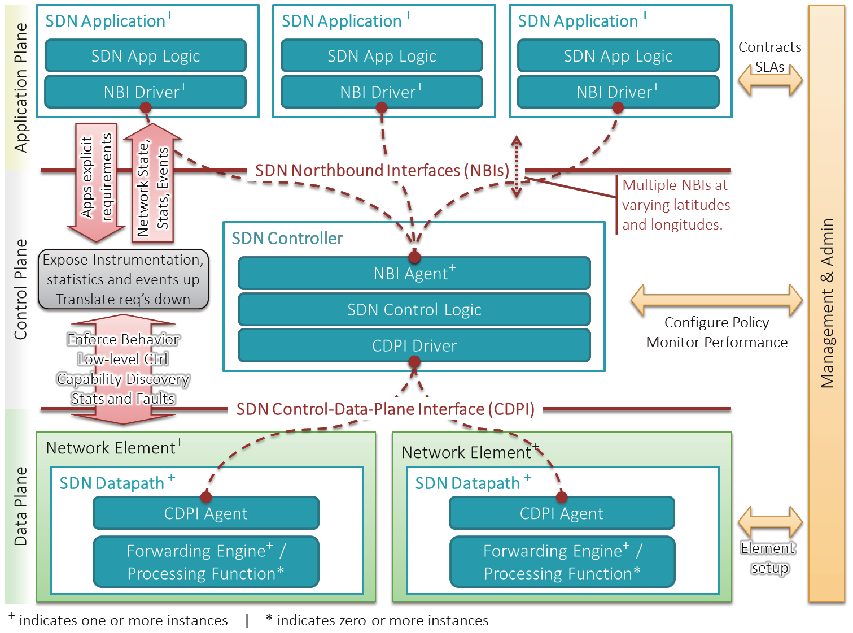
\includegraphics{arch/sdn-arch.pdf}
  \caption{软件定义网络SDN架构}
  \label{fig:pard-arch-outline}
\end{figure}


\section{本章小结}

从现有技术来看,单节点内服务质量保障技术的不足,导致节点内应用相互干扰严重,某种程
度上成为目前数据中心整体服务质量保障的短板,是成为长尾延迟现象的主要因素之一。同时
这也是一个非常具有挑战的问题,这需要跨层次协同设计。美国计算共同委员会(Computing 
Community Consortium)于2012年5月发布的计算机体系结构共同体白皮书《21世纪计算机体系
结构》中也将单节点内保障服务质量作为未来研究方向之一,其中认为[9]:“管理应用之间的相
互作用也带来了挑战。例如,这些应用如何表达服务质量(QoS)目标并且让底层的硬件、操作
系统以及虚拟层共同工作来保障它们。”

\iffalse
%%% Local Variables: 
%%% mode: latex
%%% TeX-master: t
%%% End: 

%\chapter{现有体系结构服务质量保障技术评估}
%\label{chap:curarch}

%In todays new processors the number of cores is continuously increasing
%which in turn increase the number of threads or workloads that can 
%simultaneously be run. When multi-threaded
% applications run concurrently, they compete for shared
%resources including L3 cache.  At times, this L3 cache resource contention may 
%result in inefficient space utilization. For example a higher priority thread 
%may end up with lesser L3 cache resource or a cache sensitive app may not get
%optimal cache occupancy thereby degrading the performance.
%Cache Allocation kernel patch helps provides a framework for sharing L3 cache
% so that users can allocate the resource according to set requirements.

随着多线程技术与多核平台的发展,单个节点能够提供的越来越强大的计算资源,为硬件资源共享
提供了足够的支持;而虚拟化技术的发展,特别是新兴的容器技术的出现,更加促进了硬件资源
的共享。目前,主流互联网公司已经将其部分业务迁移到了虚拟化平台或容器平台中,
能过资源共享的方式提高服务器资源利用率,但如何进行有效的任务调度依然是一个待解决的问题。
这其中最关键的两点是:实时精准的性能监控和确定性的性能隔离。
基于这一需求现有的芯片厂商都提出了自己的解决方案, % 可能只有intel的方案
如大部分芯片都支持的Performance Counter功能,可以实时监控IPC、命中率、访存带宽等功能,
Intel在E5-v3系列CPU中更是提出了Resource Director Technology(RDT)技术,
增加的对末级缓存监控(CMT)和访存带宽的监控(MBM),以及末级缓存容量划分功能(CAT)。
本章的将对这些已有技术进行分析,并讨论如何将这些技术应用到数据中心系统中以实现服务质量
保障。
% 验证Loop-back的动态调速资源分配机制的有效性

\section{实验方法介绍}

\subsection{Benchmark与应用}

使用CloudSuite和BigDataBench,代替SPEC

Intel早在多年前便在Sandy Bridge处理器中加入Way-Based的Cache Partitioning技术,
并且由UC Berkeley对该处理器进行了分析对比试验,认为Cache Partitioning能在很多
情况下提升20\%的性能。
该工作主要面向SPEC负载,但数据中心中运行的应用与SPEC存在很大差别[][],
因此在本章,希望使用现有的服务质量保障技术,对数据中心应用混合,验证其效果。

我们将应用负载分为三类:(1) Guaranteed (2) Burstable (3) Best Effort。
其中第一类是最关键的应用,需要预留足够的资源以保证其性能,对外服务基本属于些类型,
典型包括延迟敏感型的应用(如WebServer、memcache等),XXXX; % 长时在线应用
第二类是次关键的应用,它的负载会随时间出现明显的波动性,因些其资源需求也存在波动,
典型的应用包括:XXXX; % 非关键业务
第三类主要指一些可被杀死并重启的批处理应用。 % 批处理业务

调度策略是保证第一类应用,并在其中穿插后两类应用以提高利用率;实时监控第一类应用
的性能变化,对其资源进行隔离;监控第二类应用的性能变化,在必要时杀死第三类应用。

在本章中,我们以XXX做为第一类应用的代表, % WebServer, Video Stream,性能必须严格保障
XXX做为第二类应用的代表,			% Cache Server, 性能可以降低在一定范围内
XXX做为第三类应用的代表,			% Hadoop
将其混合部署到同一台服务器,并能够保障第一类应用的服务质量,同时尽可能
的保证第二类应用的性能,并在空闲时间完成第三类应用。

\subsection{实验平台}

在学术界,提出很多方案,在体系结构层次上实现性能隔离,在第\ref{chap02:}章中我们讨论了
其中主要的方案,其中Cache容量划分对性能影响较大。
Intel早在多年前便在Sandy Bridge原型处理器中加入Way-Based的Cache Partitioning技术,
UC Berkeley通过对该处理器进行了分析对比试验,认为Cache Partitioning能在很多
情况下提升20\%的性能。
在最新的E5-v3系列CPU中,Intel正式加入了对Cache容量划分的支持,本章的实验全部采用该平台。

后面将首先将对Intel的CAT/CMT技术做一简要介绍,之后将介绍如何在这一平台上构建实验环境,
并对实验目标做详细说明。


%Cache Monitoring Technology and Cache Allocation Technology provide the hardware framework to manage a shared resource, like last level cache. As multithreaded and multicore platform architectures emerge, running workloads in single-threaded, multithreaded, or complex virtual machine environment, the last level cache is a key resource to manage. Intel introduces Cache Monitoring Technology and Cache Allocation Technology to manage these various workloads across shared resources.


%同时Intel的DDIO技术中也支持将LLC中的某几个Way分配给I/O数据,
%以减少I/O数据对其他应用程序的影响。华为海思的ARM处理器也提出一定的QoS技术,
%能对LLC进行按路划分;在内存控制器增加了控制机制。
%
%虽然这些处理器带有QoS功能,但在实际应用中却并没有得到广泛的应用。
%因此,本课题将主要验证上述QoS机制的有效场景与实际效果,
%同时验证带“Loop-back”的动态调整资源分配策略机制的有效性;
%并基于电信转发控制典型业务以及互联网媒体应用,分析时延约束,流量模型及噪音影响等,
%通过X86 QoS实测数据整理出QoS特性价值地图。

\subsubsection*{ARM: Cache partition技术}

该部分需要更多的信息,如ARM64的支持。


\subsubsection*{实验平台组成}

本章所使用的实验平台由4台双路E5-v3服务器缓存,它们之间通过万兆以太网交换机互连,
如图\ref{}所示。
在该平台上部署了一个小型的Hadoop集群,HDFS配置为双副本,每个节点启用4个map和4个reduce任务;
在其上运行mahout/pagerank以及一些基于MapReduce的MicroBenchmark,做为离线应用。
同时在其中两个节点上配置了分布式的Cassandra做为分布式数据数据库实例,另外两个节点配置了
Nginx集群做为前端WebServer服务器,做为在线应用。


\section{共享缓存分析}

\subsection{缓存容量对性能影响}

递减Cache Way,对比性能,找出临界值

\subsection{缓存干扰对性能影响}

1. 运行两个应用,对比在线应用性能变化
2. 采用“限制离线应用缓存占用”策略
3. 采用“隔离在线离线应用缓存”策略

\subsection{小结}

\section{访存带宽分析}

\section{动态资源分配策略}

通过软件监控并设定阈值,对资源进行重新分配。包括Cache、CPU share等

设置不同的监控粒度,对比开销+性能变化



\section{本章小结}

通过本章研究,我们发现在没有体系结构支持的情况下,共享会存在很强烈的干扰现象,在使用
的软件隔离机制(cgroup)或调度机制后,可以在一定程度上缓解干扰。在传统体系结构下进行
扩展的新技术(如CMT/CAT),可以为共享提供一定的保障,但是需要OS或软件提供相应的支持,
因为我们需要一个新的体系结构来实现更好的服务质量保障。

\fi

